\documentclass[epsf]{article}
\usepackage{amsmath,amsthm,amsfonts,latexsym,amscd, framed}
\usepackage{graphicx}

\textwidth=6.0truein\hoffset=-.5truein
\textheight=8.5truein\voffset=-.5truein

\begin{document}
%\maketitle
\newcommand{\R}{\mathbb{R}}
\newcommand{\noi}{\noindent}
\newcommand{\bs}{\bigskip}

\newenvironment{spaced_item}{
\begin{itemize}
  \setlength{\itemsep}{5pt}
  \setlength{\parskip}{10pt}
  \setlength{\parsep}{10pt}
}{\end{itemize}}


%%%%

\begin{center}
{\Large Project \#4: Phase Portraits for Linear DE Systems\\
\vskip 2mm
TA Guide pt 2}
\end{center}

\noi{\bf 1. } I'm going to ask them to work on a couple of final exam review problems before this last section meeting -- so hopefully there will be time to discuss solutions to those as well. 
\begin{enumerate}
\item Have the students group up and compare solutions.  
\item Ask two groups to volunteer to write their solutions on the board.  
\item While they are working on that, other students can revise their answers if they feel they need to.  
\item After the solutions are up on the board, ask the students to sit down and you read/rephase/present the student solutions out loud to the class.  
\item Ask the class -- do you agree with the reasoning?  Should something more be written down?  Did anyone explain it in a different way?  Once the class is satisfied with the solutions to these problems, move on the the final exam review problems.
\end{enumerate}

\noi{\bf Problem 1} Consider the system
$$\vec{\bf x}' = \begin{bmatrix}\ \ 3 & -2 \cr -1 &\ \ 2 \end{bmatrix}\vec{\bf x}.$$
The matrix of the system has eigenvalues/vectors:
$$ \lambda_1 = 1, \ \ \vec{\bf v}_1 = \begin{bmatrix}1\cr 1 \end{bmatrix} \ \ \text{and} \ \ \lambda_2 = 4,\ \ \vec{\bf v}_2= \begin{bmatrix}-2\cr \ \ 1 \end{bmatrix}$$
\begin{itemize}
\item[(a)] Write down the general solution for the system.
\vskip 2mm 
\item[(b)] Is the equilibrium solution $\vec{\bf 0}$ a source, sink or saddle? Explain.\footnote{Please provide all of your explanations in complete sentences.}
\vskip 2mm

\item[(c)] Which eigenvector corresponds to the ``fast'' direction and which corresponds to the ``slow'' direction?  Explain how you know and how this will affect solutions trajectories as they move away from the origin.
\vskip 2mm
\item[(d)] Which of the phase portraits corresponds to this system?
\end{itemize}

\vskip 2mm

\noi{\bf Problem 2} Consider the system
$$\vec{\bf x}' = \begin{bmatrix} 1 & -1 \cr 5 & -1 \end{bmatrix}\vec{\bf x}.$$
The matrix of the system has eigenvalues/vectors:
$$ \lambda_1 = 2i, \ \ \vec{\bf v}_1 = \begin{bmatrix}1\cr 1 \end{bmatrix} + i\begin{bmatrix}0 \cr 2 \end{bmatrix}\ \ \text{and} \ \ \lambda_2 = -2i,\ \ \vec{\bf v}_2= \begin{bmatrix}1\cr 1 \end{bmatrix} - i\begin{bmatrix}0 \cr 2 \end{bmatrix}$$

\begin{itemize}
\item[(a)] Write down the general solution for the system.
\vskip 2mm
\item[(b)] Are solution trajectories in the phase plane oscillating?  Are they periodic? Explain how you can tell.
\newpage

\item[(c)] Since the eigenvalues are complex, there should be some sort of rotation in the phase plane.  Will this rotation be clockwise or counterclockwise?  Explain how you can tell.
\vskip 2mm
\item[(d)] Which of the phase portraits corresponds to this system?
\end{itemize}


\noi{\bf 2. } I've asked the class to work on problems \#1, \#6 and \#7 \textit{before} section on Wednesday.  Hopefully you will have time to discuss solutions to these three problems:

\begin{itemize}

\item[1.] Consider the forced spring-mass system governed by the equation $$y''+ 2y' +2y = 2\cos(t)$$

\noi (a) What is the mass of the object, the damping coefficient, the spring constant and the external force for this system?
\vskip 2mm

\noi (b) Find the general solution to the differential equation.  Identify the fundamental set for solutions to the corresponding homogeneous equation and the particular solution to the nonhomogeneous equation that appears in your general solution.
\vskip 2mm

\noi (c) Find \textit{a different} fundamental set for solutions to the homogeneous equation and \textit{a different} particular solution and express the general solution in terms of these functions.
\vskip 2mm

\noi (d) Solve the DE with initial conditions $y(0) = 2$ and $y'(0) = 0$.
\end{itemize}

\noi{\bf 3. } If you want to solve the DE for them in the interest of saving time - that might work better.  Once you get to part (c) give them a few minutes to think about what to do to get the ``different'' solution.  Many of them will think they have to use variation of parameters (which is a huge pain for this problem).  The more clever approach is to pick another basis for the fundamental set and to pick a different particular solution.  Mostly I want them to realize what this affine structure really means.  Someone in the class may see the slick way to do it - if they don't, show them.\\

\begin{itemize}
 \item[6.] Given the following general linear 2nd order differential equations:
\begin{align*}
y'' +p(t)y' +y &= f(t) \ \ \ \text{(N)}\\
y'' +p(t)y' +y &= 0\ \ \ \ \ \ \ \text{(H)}
\end{align*}
Which of the following statements are true.  Circle \textit{all} that apply.
\begin{itemize}
\item[A.] If $y_1$ and $y_2$ are solutions to (N), then $y_1+y_2$ is a solution to (N).
\item[B.] There is only one possible particular solution to (N).
\item[C.] If $y_1$ and $y_2$ are solutions to (N), then $y_1 - y_2$ is  a solution to (H).
\item[D.] The solution space for (N) is a vector space ``shifted'' by a particular solution to (N).
\end{itemize}


\item[7.] Given the following $2\times 2$ linear system with constant coefficients
\begin{align*}
\vec{\bf x} ' &= A\vec{\bf x} \ \ \ \ \ \ \ \ \ \ \ \ \ \text{(H)}\\
\vec{\bf x} ' &= A\vec{\bf x} + \vec{\bf f}(t), \ \ \  \text{(N)}
\end{align*}
where $\vec{\bf f}$ is not the zero vector-function.  Which of the following statements are true.  Circle \textit{all} that apply.
\begin{spaced_item}
\item[A.] If $\vec{x}_h$ is a solution to (H) and $\vec{x}_p$ is a solution to (N), then $\vec{x}_h + 2\vec{x}_p$ is a solution to (N).
\item[B.] If $\vec{x}_1$ and $\vec{x}_2$ are both solutions to (N), then $\vec{x}_1- \vec{x}_2$ is a solution to (H).
\item[C.] There is only one possible particular solution to (N). 
\item[D.] The solution space to (N) is a 2-dimensional vector space.
\end{spaced_item}

\end{itemize}

\noi{\bf 4. } These two multiple choice problems are essentially the same.   Talk through the solution to \#6, then build on those ideas to explain the solutions to \#7.  I'm hoping the students will see how these ideas are connected.\\

\newpage

Use the following phase portraits to answer part (d) of problems 1 and 2. \\


\begin{center}
A 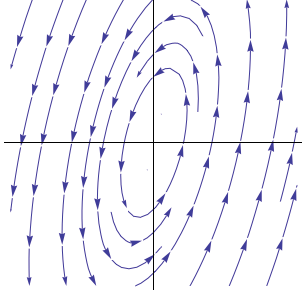
\includegraphics[width=40mm]{center1.png}\hspace{0.6 cm}B 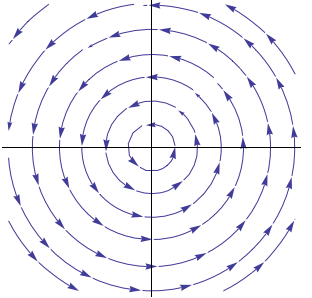
\includegraphics[width=40mm]{center2.png}\hspace{0.6cm}C 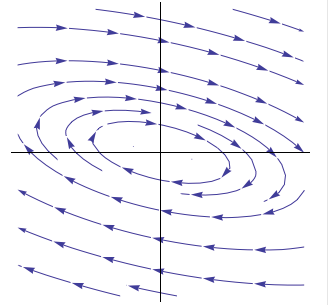
\includegraphics[width=40mm]{center3.png}\\

\vskip 1cm
D 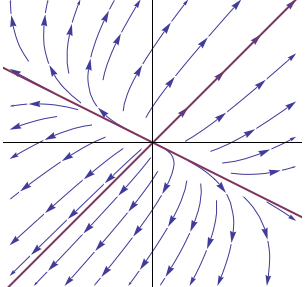
\includegraphics[width=40mm]{source1.png}\hspace{0.6 cm} E 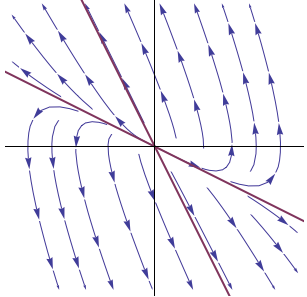
\includegraphics[width=40mm]{source2.png}\hspace{0.6 cm} F 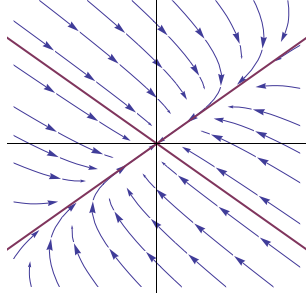
\includegraphics[width=40mm]{sink.png}\\
\vskip 1cm
G 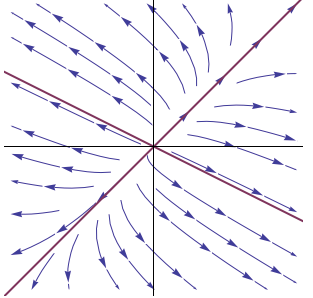
\includegraphics[width=40mm]{source4.png}\hspace{0.6 cm} H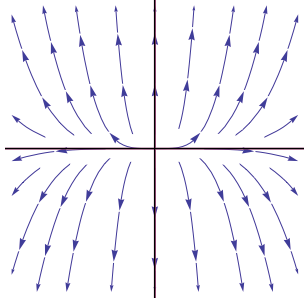
\includegraphics[width=40mm]{source3.png}\hspace{0.6 cm} I 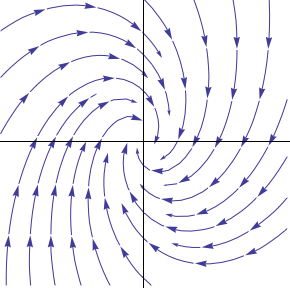
\includegraphics[width=40mm]{stable_spiral.png}\\
\vskip 1cm
J 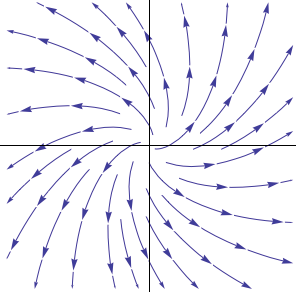
\includegraphics[width=40mm]{spiral_source.png}\hspace{0.6 cm} K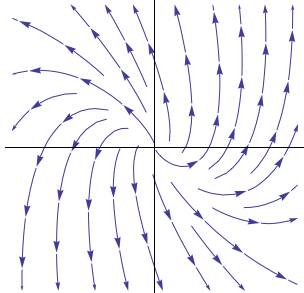
\includegraphics[width=40mm]{spiral_source2.png}\hspace{0.6 cm} L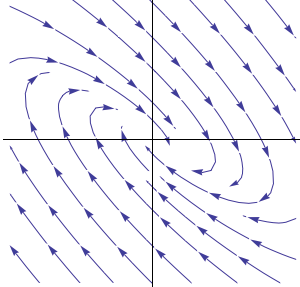
\includegraphics[width=40mm]{stable_spiral2.png}\\
\end{center}

\end{document}
%%%%%%%%%%%%%%%%%%%%%%%%%%%%%%%%%%}

\begin{enumerate}
\item Next we consider a more challenging system
\begin{equation}
\label{N2}
\vec{x}' =\begin{bmatrix}1 & 1 \cr 4 & 1 \end{bmatrix}\vec{x} + \begin{bmatrix} 2t \cr 0 \end{bmatrix}.
\end{equation}

\vskip 2mm

\noindent (a) By writing (\ref{N2}) in the right coordinates, we \textit{decouple} the system and can easily solve it.  Let $\mathcal{B} = \{\vec{v}_1, \vec{v}_2 \}$, where 
$$\vec{v}_1 := \begin{bmatrix}1 \cr 2 \end{bmatrix} \text{ and } \vec{v}_2 := \begin{bmatrix}\ \ 1 \cr -2 \end{bmatrix}$$ 
are linearly independent eigenvectors of the matrix $A = \begin{bmatrix}1 & 1 \cr 4 & 1 \end{bmatrix}$.  Let $\vec{w}:= (\vec{x})_{\mathcal{B}}$ and write down the system for $\vec{w}$ - you should get a (very familiar) decoupled nonhomogeneous system.  What is $\vec{w}(t)$?

\vskip 2mm
\noindent (b) Use a change-of-coordinates to compute $\vec{x}(t)$.

\vskip 2mm
\noindent (c) Since this is one of the first nonhomogeneous system you've solved, I strongly suggest that you verify that your solution $\vec{x}$ satisfies the original system (\ref{N2}).

\vskip 2mm
\noindent (d) Describe the solution space for (\ref{N2}).\\

\item Solve the following nonhomogeneous systems by decoupling them.
\vskip 2mm
\noi (a) $$\vec{\bf x}' = \begin{bmatrix} 2 & -1 \cr 3 & -2  \end{bmatrix} \vec{\bf x} + \begin{bmatrix}e^t \cr t \end{bmatrix}.$$
\vskip 2mm

\noi(b) For this one, you will have to work with complex coordinates. $$\vec{\bf x}' = \begin{bmatrix} 2 & -5 \cr 1 & -2  \end{bmatrix} \vec{\bf x} + \begin{bmatrix}-\cos t \cr \sin t\end{bmatrix}.$$\\

\item For the homogeneous system
\begin{equation}
\label{J}
\vec{x}' = \begin{bmatrix}\ \ 2 & 1 \cr -1 & 4 \end{bmatrix}\vec{x},
\end{equation}  
decoupling hits a snag: The matrix $B := \begin{bmatrix}\ \ 2 & 1 \cr -1 & 4 \end{bmatrix}$ does not have two linearly independent eigenvalues, so $B$ cannot be diagonalized (and the system cannot be solve our usual way).  However, the matrix can be put in the \textit{Jordan form}:
\begin{equation*}
J = \begin{bmatrix}\lambda & 1\cr 0 & \lambda \end{bmatrix}
\end{equation*} 
where $\lambda$ is the eigenvalue for $B$.  To do this we must change the coordinates for $B$ to the basis $\mathcal{B} = \{\vec{v}, \vec{u} \}$ where $\vec{v}$ is an eigenvector associated with the eigenvalue $\lambda$ and $\vec{u}$ is a solution to the equation $(A - \lambda I)\vec{u} = \vec{v}$.  We call   $\vec{u}$ a \textit{generalized eigenvector} of $B$.
\vskip 2mm
\noindent (a) Compute $\lambda$, $\vec{v}$ and $\vec{u}$ and verify that $[B]_{\mathcal{B}} = J$.

\vskip 2mm
\noindent (b) Show how you can use a modified decoupling method to solve the system (\ref{J}).

\vskip 2mm
\noindent (c) It's a good idea to double check your solution to (\ref{J}) now.

\end{enumerate}
\end{document}
